\subsection{UC-9}
\label{subsec:UC-9}

\begin{figure}[H]
    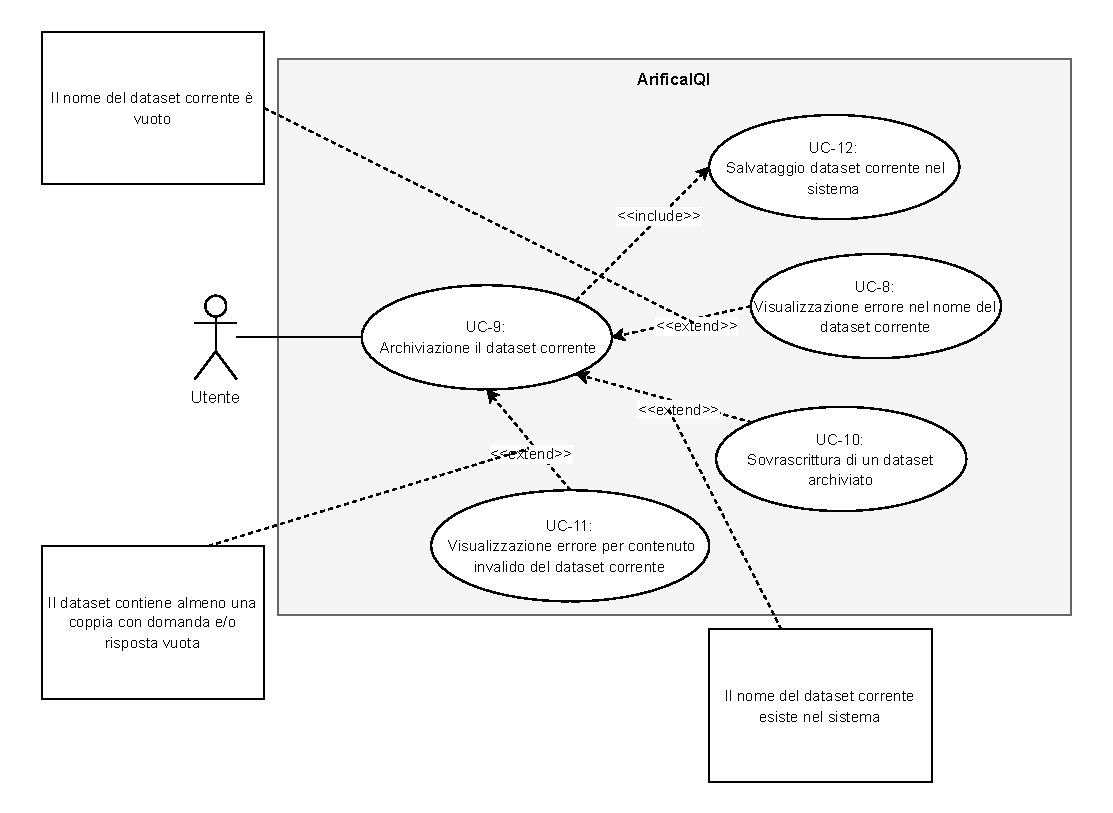
\includegraphics{Sezioni/UseCase/Immagini/UC-9.pdf}
    \caption{Diagramma UC-9.}
\end{figure}

\begin{usecase}{UC-9}{Visualizzazione dei dataset archiviati}
    \req{\hyperref[item:RU-3]{RU-3}} 

    \pre{
        \item Il sistema è attivo e funzionante
    }

    \post{
        \item L'utente conosce la lista dei dataset archiviati
    }
    
    \actor{Utente}

    \subactors{}

    \trigger{L'utente deve visualizzare i dataset archiviati}
    
    \inc{}

    \base{}

    \scenario{
        \item L'utente richiede la visualizzazione dei dataset archiviati
        \item Viene visualizzata la lista dei dataset archiviati in ordine lessicografico
    }

    \subscenario{
        \item[1.1] \textbf{Non esistono dataset archiviati}
        \begin{itemize}
            \item [a.] Viene indicato all'utente che non esistono dataset archiviati
        \end{itemize}
    }
\end{usecase}